\documentclass{article}
\usepackage{amsmath}
\usepackage{breqn}
\usepackage{amssymb}

\usepackage{geometry}
\geometry{margin=1in}

\usepackage{hyperref}
\hypersetup{
    colorlinks=true,
    linkcolor=black,
    filecolor=magenta,      
    urlcolor=cyan,
    pdfpagemode=FullScreen,
}

\usepackage{wrapfig}
\usepackage{graphicx}
\graphicspath{ {./images/} }

\setcounter{secnumdepth}{4}
\setcounter{tocdepth}{4}

\makeatletter
\newcommand\subsubsubsection{\@startsection{paragraph}{4}{\z@}{-2.5ex\@plus -1ex \@minus -.25ex}{1.25ex \@plus .25ex}{\normalfont\normalsize\bfseries}}
\newcommand\subsubsubsubsection{\@startsection{subparagraph}{5}{\z@}{-2.5ex\@plus -1ex \@minus -.25ex}{1.25ex \@plus .25ex}{\normalfont\normalsize\bfseries}}
\makeatother


\begin{document}
\begin{titlepage}
    \begin{center}
        \vspace*{1cm}
            
        \Huge
        \textbf{Playing draughts using reinforcement learning}
            
        \vspace{0.5cm}
        \LARGE
        A deep learning model that plays draughts via a neural network library with auto differentiation - built from scratch
            
        \vspace{1.5cm}
            
        \textbf{Edgar Maddocks}
            
        \vfill
            
        \vspace{0.8cm}
                        
        \Large
        Bedford School\\
        03/05/2024\\
            
    \end{center}
\end{titlepage}

    \pagebreak

    \tableofcontents

    \section{Analysis}
    \subsection{Background}
    \textbf{TO BE WRITTEN}

    \subsection{Evidence of Analysis}

    \subsubsection{Current systems}

    \subsubsubsection{Draughts}
    Draughts is an English board game played on an 8x8 checkered board, identical to a chessboard.
    Each player begins a game with 12 pieces, usually flat round discs.
    The pieces and board are usually black and white, and will be referred to as such.
    The board is first placed between the two players such that the bottom right-hand corner is a white square,
    for both players.
    
    A coin is tossed to decide who plays black, and that player has the first move. Each player places their pieces
    on the 12 black squares closest to themselves. The setup of the board can be seen in Figure 1. 

    \begin{wrapfigure}[11]{l}{0.4\linewidth}
        \centering
        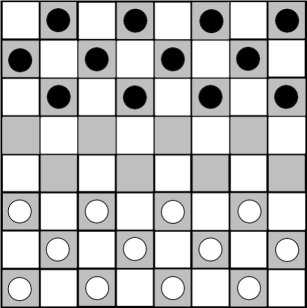
\includegraphics[scale=0.35]{The-starting-position-for-checkers.png}
        \caption{An image showing the starting position of a game of draughts}
    \end{wrapfigure}

    The pieces only move diagonally (so will always be on black squares)
    and the aim is to take all of the opposing players pieces, or to put the opposing player in a position with no possible moves.
    Players take turns moving their shade of pieces. If at any point of the game, a player's piece reaches the opposing players edge
    of the board, the piece becomes a 'King', and another piece should be placed on top of said piece to indicate so.

    Unless a piece is crowned and a 'King' it may only move and take pieces diagonally forwards. Kings may move and take both forwards and backwards.
    \begin{wrapfigure}[15]{r}{0.4\linewidth}
        \centering
        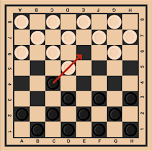
\includegraphics[scale=1.15]{piece being taken.png}
        \caption{Example of a piece being taken in draughts}
    \end{wrapfigure}

    If an adjacent square has an opponents piece and the square immediately beyond the oppositions piece is empty, the opponents piece may be captured.
    If the player who's go it is has the opportunity to capture one or more pieces, then they must do so. 
    A piece is taken by moving your own piece over the opposing player's, into the vacant square, and then removing the opposing piece from the board.
    An example of this process can be seen in Figure 3.

    Unlike a regular move, a capturing move may make more than one 'hop'. This is if the capture places the piece in a position where another capture is possible.
    In this case, the additional capture must be made. The capture sequence can only be made by one piece per move. i.e. You cannot make one capture with one piece, 
    and then another capture with another piece in the same move.
    
    However, if more than one piece can capture, the player has free choice over which piece to move. Likewise, if one piece can capture in multiple
    directions then the player has the choice in which direction to move. \textbf{Note:} it is not compulsory for the player to move in the direction, or with the piece,
    that will lead to the greatest number of captures in that move.
    
    \begin{wrapfigure}[16]{l}{0.4\linewidth}
        \centering
        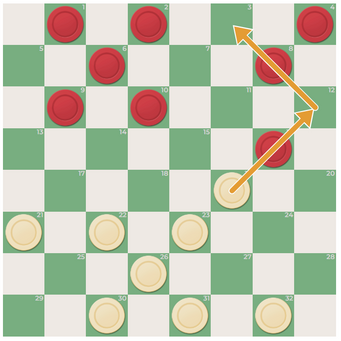
\includegraphics[scale=0.8]{double hop.png}
        \caption{Visualization of multiple captures in one move}
    \end{wrapfigure}

    A move may only end when the position has no more captures available or an uncrowned piece reaches the opposing edge
    of the board and becomes a King. 

    If no capturing moves can be made, then any piece may be moved diagonally onto a vacant square.

    The game ends when all of a players piece's have been captured, or a player has no available moves.

    \subsubsubsection{Neural Networks}
    \subsubsubsubsection{What is a neural Network}
    A neural network is a machine learning model which aims to mimic the processes of the human brain.
    Each network contains inputs and outputs, as well as one or more layers of hidden nodes - which act as artificial neurons.
    In a fully connected network, each node is connected once to each node in the next layer - an example of how one node connects
    to the next layer can be seen in below.
    \begin{figure}[h]
        \centering
        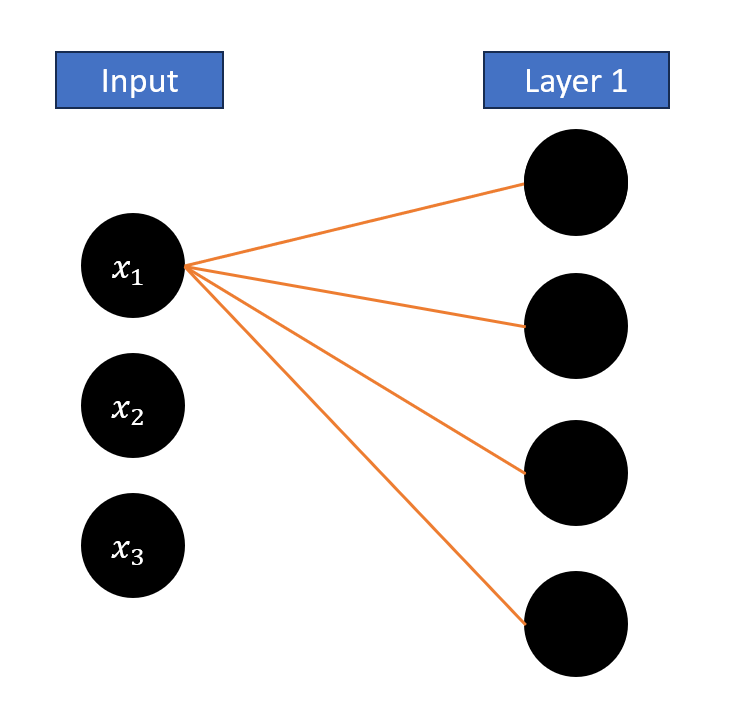
\includegraphics[scale=0.2]{ConnectedNode.png}
        \caption{Example of a fully connected node and layer}
    \end{figure}

    Neural networks are a supervised learning model, meaning that they learn from labeled data (which has the objective correct answer in the data).
    They are sometimes referred to as artificial neural networks (ANNs) or simulated neural networks (SNNs).\\

    Neural networks can be modelled as a collection linear regression units.

    \subsubsubsubsection{Linear Regression Unit}
    A single linear regression unit output has the formula:
    \begin{displaymath}
        \hat{y} = \sum_{i=0}^{n} w_ix_i + b
    \end{displaymath}

    Where $\hat{y}$ is the predicted output, $n$ is the number of inputs, $x_i$ is the $i$th input, $w_i$ is the weight of $x_i$, and $b$ is a bias.
    If, for example, there were 3 inputs the full equation for $\hat{y}$ would be:
    \begin{displaymath}
        \hat{y} = w_1x_1 + w_2x_2 + w_3x_3 + b
    \end{displaymath}

    \subsubsubsubsection{Vectorization of processes}
    This calculation can be vectorized to improve efficiency and would be notated:
    \begin{displaymath}
        \hat{y} = XW + b
    \end{displaymath}

    Where we let
    \begin{displaymath}
        W = \begin{bmatrix}
            w_1\\
            w_2\\
            \vdots\\
            w_n
        \end{bmatrix}\\
        \hspace{25px}
        X = \begin{bmatrix}
            x_1&
            x_2&
            \hdots&
            x_n
        \end{bmatrix}
    \end{displaymath}

    $X$ here is a row vector as this is the most common format for data as an input to a network (e.g being read from a csv).
    This parallelized computation is much faster, and can be parallelized using the GPU to further improve speed and efficiency.

    \subsubsubsubsection{Forward Pass of Dense Layer}
    In the case of neural networks, lots of these linear regression units can be combined to form a vector of outputs.
    Each of these regression units will have the same inputs, therefore $X$ can have the same definition. However, $W$ will now be
    composed of multiple vectors of weights, instead of just one.

    Here we let
    \begin{displaymath}
        W = \begin{bmatrix}
            w_{11} & w_{21} & \dots & w_{j1}\\
            w_{12} & w_{22} & \dots & w_{j2}\\
            \vdots & \vdots & \ddots & \vdots\\
            w_{1n} & w_{2n} & \dots & w_{jn}
        \end{bmatrix}
    \end{displaymath}

    Where $j$ is now the number of nodes in the layer. If we rewrite our forward pass equation to use this weight matrix,
    with each node as its own regression unit:
    \begin{displaymath}
        Y = XW + B
    \end{displaymath}

    Where:
    \begin{displaymath}
        Y = \begin{bmatrix}
            \hat{y_1}&
            \hat{y_2}&
            \hdots&
            \hat{y_n}
        \end{bmatrix} \hspace{15mm}
        B = \begin{bmatrix}
           b_1 & b_2 & \dots & b_j
        \end{bmatrix}
    \end{displaymath}

    With $W$ and $X$ having the same definition as most recently defined.

    \subsubsubsubsection{Gradient Descent}

    Now, to update the weights of our model, we can compute these values in closed form, however, it comes with a large time complexity (greater than $O(n^3)$), and therefore
    a process called gradient descent is usually employed.

    Gradient descent works to minimize the error of a model by iteratively locating a minimum in the error function.
    For example, a common cost (error) function is mean squarred error.
    \begin{displaymath}
        MSE(Y, \hat{Y}) = \frac{1}{n}\sum_{i=0}^{n}\left(y_i - \hat{y}_i\right)^2
    \end{displaymath}

    This function effectively calculates the absolute distance between the predicted value of one data point ($\hat{y_i}$) and the true value at that same point ($y_i$),
    for every value in the dataset (of size $n$) and takes the mean of these distances.
    Again, this calculation can be vectorized using the equation below.
    \begin{displaymath}
        MSE(Y, \hat{Y}) = \frac{1}{n}((Y - \hat{Y})^T \cdot (Y - \hat{Y}))
    \end{displaymath}

    If we plot the MSE curve of different weights and biases - of a single regression unit, it looks as follows.
    \begin{figure}[h]
        \centering
        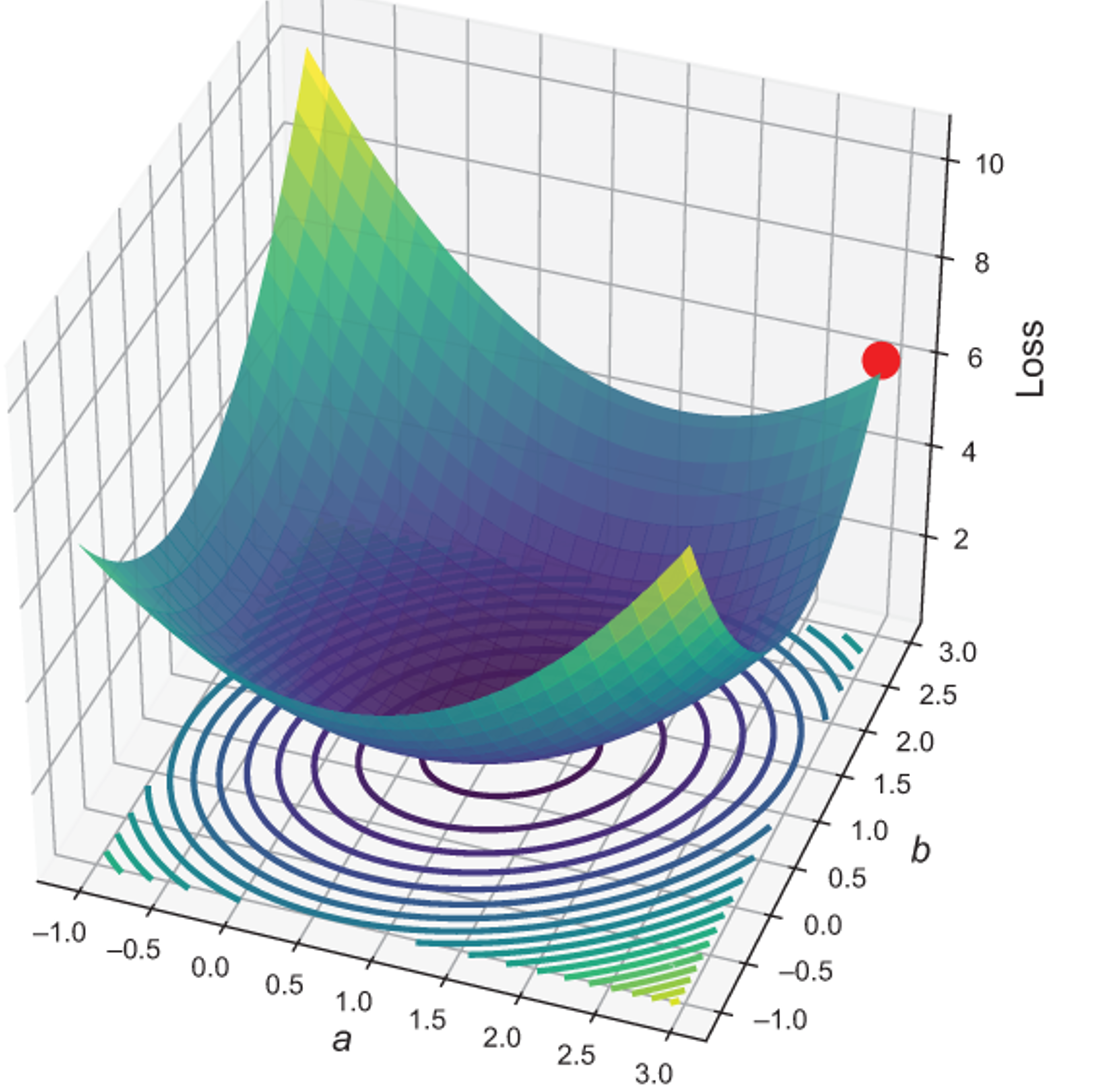
\includegraphics[scale=0.5]{MSEplot.png}
        \caption{Plot of MSE in a single regression unit}
    \end{figure}

    Here the weight has been labelled $a$, but the bias has remained as $b$. As we can see, there is a clear local minimum of this error function,
    and the values that obtain this minimum, is what gradient descent aims to achieve. 
    \begin{wrapfigure}[14]{l}{0.4\linewidth}
        \centering
        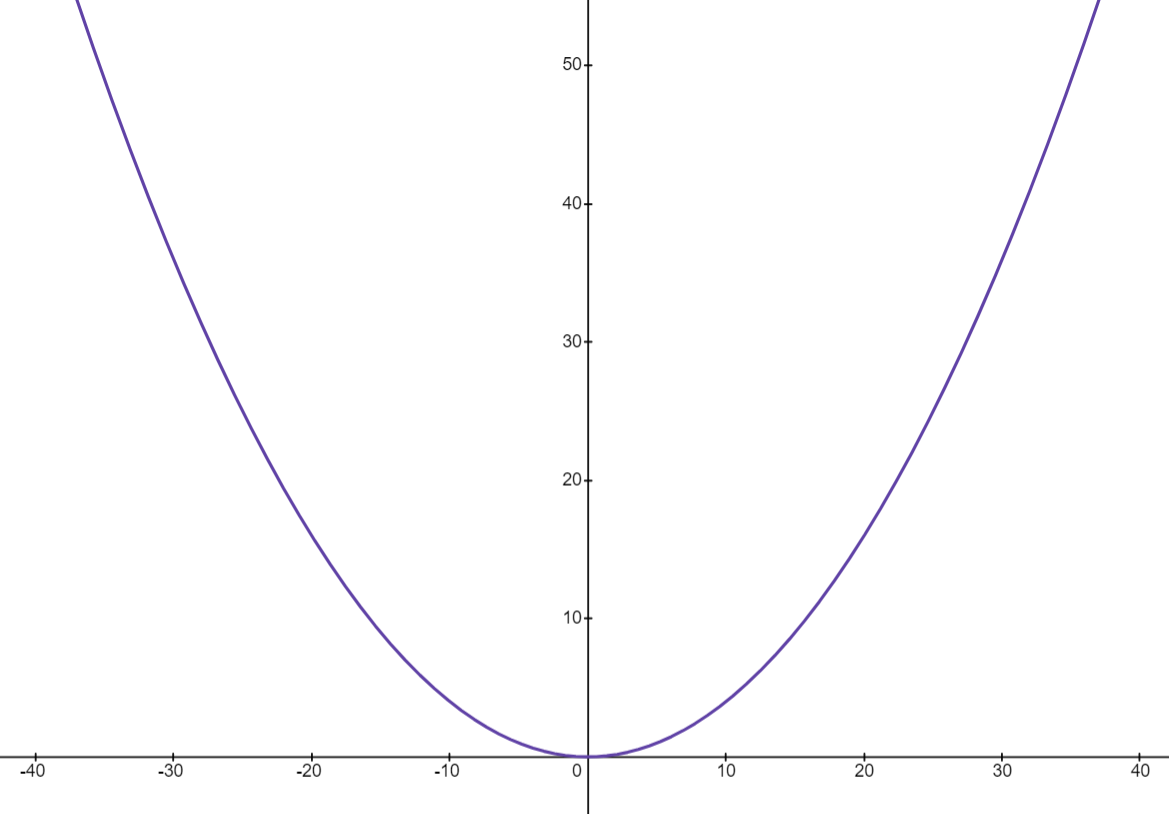
\includegraphics[scale=0.2]{image.png}
        \caption{MSE with respect to one parameter}
    \end{wrapfigure}

    In figure 6 we can see a representation of the MSE plot with respect to only one of the parameters. This makes understanding the process of gradient
    descent much simpler. For example, the minimum of this function ($f(x) = \frac{x^2}{25}$) is at $x = 0$. So, if we were to have an initial $x$ value of say $-40$
    and we calculated the gradient to be $3.2$, we could then subtract this from $40$. Resulting in a new value of $36.8$, which is closer to our optimal value of $0$.
    This process is completed iteratively until the minimum, or near to it, is reached.

    To denote this mathematically, we can say that 
    \begin{align}
        w_{t+1} = w_t - \alpha \frac{\partial E}{\partial w}\\
        b_{t+1} = b_t - \alpha \frac{\partial E}{\partial b}
    \end{align}

    Where $w_{t+1}$ and $b_{t+1}$ are the parameters at the next timestep, $w_t$ and $b_t$ is the value of the parameters at the current timestep, 
    $\frac{\partial E}{\partial w}$ and $\frac{\partial E}{\partial b}$ are the derivatives of the error with respect to each parameter, 
    and $\alpha$ is the learning rate. This learning rate controls the size of our 'jumps' and prevents the process from beginning to spiral away
    from the optimal values.

    That is a basic overview of gradient descent in a single regression unit, but in a dense network, the process is almost identical. An error function is evaluated, 
    the derivative with respect to the inputs calculated, and the new values updated. The main expense computation-wise is calculating all of the derivatives, with respect to
    each set of parameters, as this requires passing the output from the error function backwards through all of the layers and processes. To combat this, automatic differentiation
    can be used, which tracks computation dynamically at run time to compute derivatives.

    \subsubsubsection{Automatic Differentiation}
    As mentioned, automatic differentiation tracks computation dynamically and then computes derivatives using a computational graph. This allows models to
    have much more complex forward passes, including decision branches and loops where the length of the loop is decided at runtime.

    Automatic differentiation operates by differentiating a complex function (that we don't know the derivative of), by treating it as a composition of more elementary functions
    (of which we do know the derivatives). Additionally, it treats each of these elementary functions as though their output is an intermediate variable when computing the
    complex function. This becomes very useful when there are multiple inputs to the function, and we only want the derivative to one of these variables. Finally, this process
    makes use of the chain rule to compute the derivative with respect to the inputs, as will be shown later on.

    Firstly, I will walkthrough an example of the process of automatic differentiation.\\
    \noindent Say we have a function: \begin{displaymath}
        f(x) = ln\left(\frac{sin(x_1)}{cos(x_2)}\right)
    \end{displaymath}

    This function has two arbitrary inputs (perhaps in the case of a neural network these could be our parameters or outputs for example). At first, this is quite a complex
    function to differentiate but we can simplify it using intermediate variables. For example \begin{align}
        v_1 &= sin(x_1)\\
        v_2 &= cos(x_2)\\
        v_3 &= \frac{v_1}{v_2}\\
        v_4 &= ln(v_3)\\
        y &= v_4
    \end{align}

    \begin{wrapfigure}[19]{l}{0.5\linewidth}
        \centering
        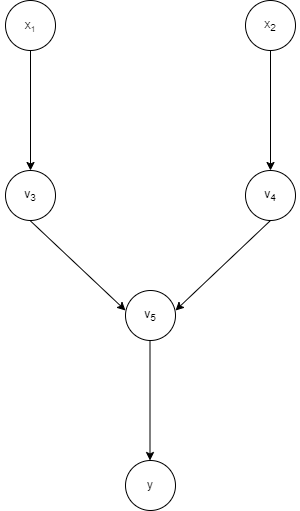
\includegraphics[scale = 0.34]{ExampleCompGraph.png}
        \caption{Example Computational Graph}
    \end{wrapfigure}
    Now that we have declared our intermediate variables, we can see how automatic differentiation splits up the original function into elementary ones.
    This then allows use to easily take derivatives. Firstly, we can draw out the computational graph for this function, using our intermediate variables,
    and this can be seen in Figure 7.
    This graph visualizes the forward pass of the function, and how the intermediate varibales compose to form our original function.

    Now, when we want to take the derivative with respect to one of these inputs, we can simply reverse through the graph, taking the gradient of each intermediate
    variable, and using the chain rule to give us our final derivative.

    This process would looks as follows: \begin{align}
        \frac{\partial y}{\partial x_1} = \frac{\partial y}{\partial v_4} \cdot \frac{\partial v_4}{\partial v_3} \cdot \frac{\partial v_3}{\partial v_1} \cdot \frac{\partial v_1}{\partial x_1}
    \end{align}

    If we computed each of these derivatives:
    \begin{align}
        \frac{\partial y}{\partial v_4} &= 1\\
        \frac{\partial v_4}{\partial v_3} &= \frac{1}{v_3}\\
        \frac{\partial v_3}{\partial v_1} &= \frac{1}{v_2}\\
        \frac{\partial v_1}{\partial x_1} &= cos(x_1)
    \end{align}

    And finally, evaluating equation $(8)$, as well as substituting our intermediate variables in terms of $x_1$, to obtain $\frac{\partial y}{\partial x_1}$:
    \begin{align}
        \frac{\partial y}{\partial x_1} &= \frac{cos(x_1)}{v_3 \cdot v_2}\\
        &= \frac{cos(x_1)}{v_1}\\
        &= \frac{cos(x_1)}{sin(x_1)}
    \end{align}

    This process of traversing through the graph backwards is known as reverse accumulation auto differentiation, and in practice each of the gradients would be
    stored numerically at computation, rather than computing a symbolic version of the final derivative and plugging the values in.

    \subsubsubsection{Reinforcement Learning (RL)}

    \subsubsection{Similar Systems}
    \begin{wrapfigure}[13]{r}{0.5\linewidth}
        \centering
        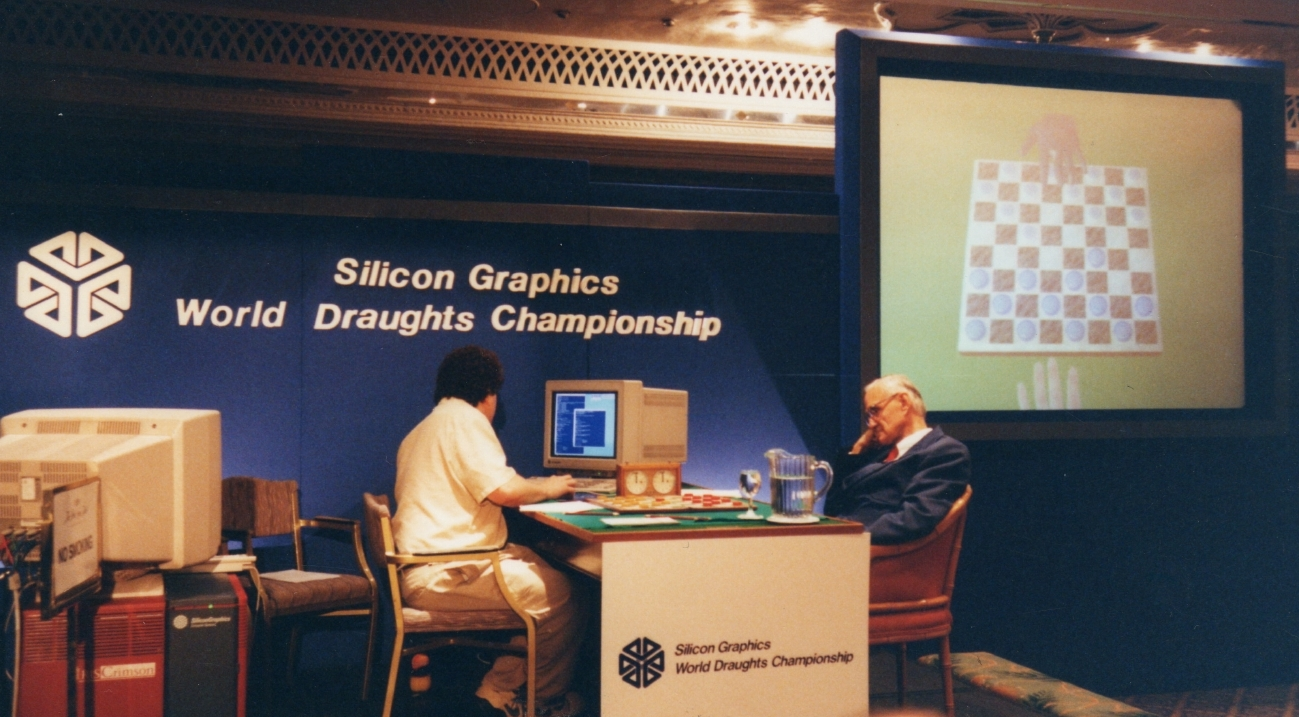
\includegraphics[scale=0.145]{1992Tinsleymatch.jpg}
        \caption{Image of Chinook playing a game of draughts - 1992}
    \end{wrapfigure}

    Chinook is a checkers playing computer program that was developed at the University of Alberta between
    1989 and 2007. The program utilises an opening book, deep-search algorithms alongside a position evaluation function
    and a solved endgame database for positions with 8 pieces or fewer.
    All of Chinook's knowledge has been programmed in by humans, with no use of an artificial intelligence model. Despite this,
    Chinook managed to beat the draughts world champion at the time of 1995, and after this no longer competed, but instead was
    tasked with solving checkers. (A solved game is one where the outcome can be predicted from any position). Finally, in 2007,
    Chinook had solved checkers, and this was published.

    \begin{wrapfigure}[12]{l}{0.5\linewidth}
        \centering
        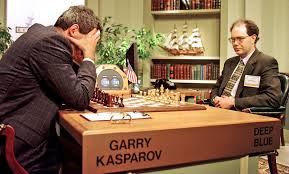
\includegraphics[scale=0.75]{download.jpg}
        \caption{Chess champion Garry Kasparov loses to Chess engine - 1997}
    \end{wrapfigure}
    Other similar systems include chess engines - of which there is a multitude. Chess engines operate similarly to Chinook, creating trees
    of possible moves and using a minimax algorithm, as well as alpha-beta pruning to determine the best move. Additionally, there are some
    chess engines which use reinforcement learning, such as Google DeepMind's AlphaZero engine. This engine has also been trained on games
    such as Go and Shogi. AlphaZero is trained mainly using self-play, where the AI plays against itself and then learns from those games.
    In a 100 game match against StockFish (one of the most popular chess engines) AlphaZero won 28 games, lost 0 and drew the remaining 72.
    This shows the power of reinforcement learning as a tool for board games and its possibility to be used for draughts.
    \vspace{5mm}

    For automatic differentiation, some of the most popular systems include PyTorch's autograd, as well as autodiff by JAX. PyTorch has a very
    well developed library for deep-learning alongside it's autograd, as well as extensive documentation. Additionally, autograd is more similar
    to regular python than JAX and may be easier to use when first delving into the area. However, JAX builds on top of autograd and accelerates
    the linear algebra using its XLA backend. This backend optimizes operations for CPU's GPU's and TPU's as well as using a just-in-time compiler
    to increase computation speeds.

    \subsubsection{Identification of end-user}
    \textbf{TO BE WRITTEN}
    
    \subsection{Modelling of the problem}
    \textbf{TO BE WRITTEN}
    
    \subsubsection{Identification of Objects}
    \textbf{TO BE WRITTEN}

    \subsubsection{Identification of Data Structures}
    \textbf{TO BE WRITTEN}

    \subsection{Set of objectives}
    \textbf{TO BE WRITTEN}
    
    \section{Research Log}

    \subsection{Draughts Rules}
    \url{https://www.mastersofgames.com/rules/draughts-rules.htm}

    \subsection{Neural Networks}
    \noindent \url{https://www.ibm.com/topics/neural-networks}

    \subsubsection{Vectorization of summations}
    \noindent \url{https://courses.cs.washington.edu/courses/cse446/20wi/Lecture8/08_Regularization.pdf}
    
    \subsection{Automatic Differentiation}
    \noindent \url{https://en.wikipedia.org/wiki/Automatic_differentiation}

    \subsection{Implementing Custom Classes using Numba}
    \noindent \url{https://numba.pydata.org/numba-doc/latest/extending/interval-example.html}
    Numba does not allow user-declared classes and therefore they must be explicity defined using Numba's types.

    \subsection{AlphaZero}
    \noindent \url{https://ai.stackexchange.com/questions/13156/does-alphazero-use-q-learning}
    \noindent \url{https://suragnair.github.io/posts/alphazero.html}
    Explanations of AlphaZero's loss function

    \noindent \url{https://liacs.leidenuniv.nl/~plaata1/papers/CoG2019.pdf}
    AlphaZero policy explanation

    \subsection{Existing Auto differentiation systems}
    \noindent \url{https://medium.com/@utsavstha/jax-vs-pytorch-a-comprehensive-comparison-for-deep-learning-10a84f934e17}
    PyTorch vs JAX
\end{document}